\section{Sensor Principle}
\label{sec:functionality}
%\note{The operating principles of 2D TMD and 2D TMD heterojunction gas sensors are explained. High surface-to-volume ratio $\rightarrow$ 2D material behaves differently than bulk material (increased reactivity) $\rightarrow$  analyte gas donates/accepts electrons from 2D film $\rightarrow$  carrier density of 2D film is modulated $\rightarrow$  measurable resistance change }
2D \gls{tmd} gas sensor can be categorized as chemiresistors. This means that the electrical resistance of the structure is modulated by the chemical environment of the sensor. Due to the extreme surface to volume ratio of these structures, this effect is especially pronounced, as the chemical interaction is primarily a surface effect. The resistance modulation effect is based on gas molecules adsorbing onto the surface of the sensor. Depending on the basicity/acidity of the gas, it is donating/accepting electrons from the 2D material. This charge transfer effects the density of holes and electrons, which, according to the formula $\sigma = n\mu_e + p\mu_h$, affects the conductivity. $\sigma$ refers to the electrical conductivity, $n$ to the electron densitivy, $\mu_e$ to the electron mobility, $p$ to the hole density, and $\mu_h$ to the hole mobility. In bulk materials, this interaction would only cause surface effects. Since 2D materials have no bulk that could dampen this effect, the conductivity modulation is especially pronounced. \Cref{fig:sensor_principle} shows a depiction of this behavior. 

\begin{figure}
\centering
\begin{subfigure}{0.49\textwidth}
    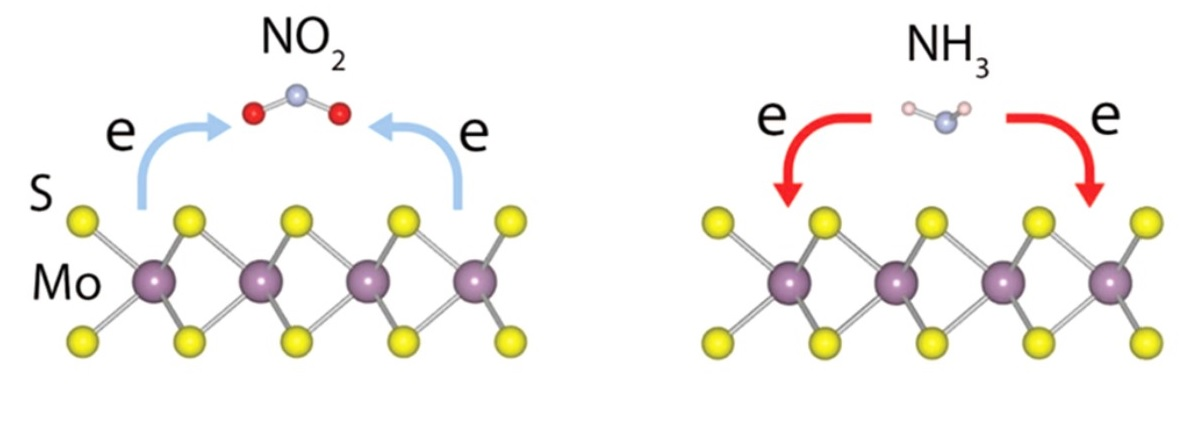
\includegraphics[width=\textwidth]{02_functionality/fig/adsorption.jpg}
    \caption{}
    \label{fig:adsorption_process}
\end{subfigure}
\begin{subfigure}{0.49\textwidth}
    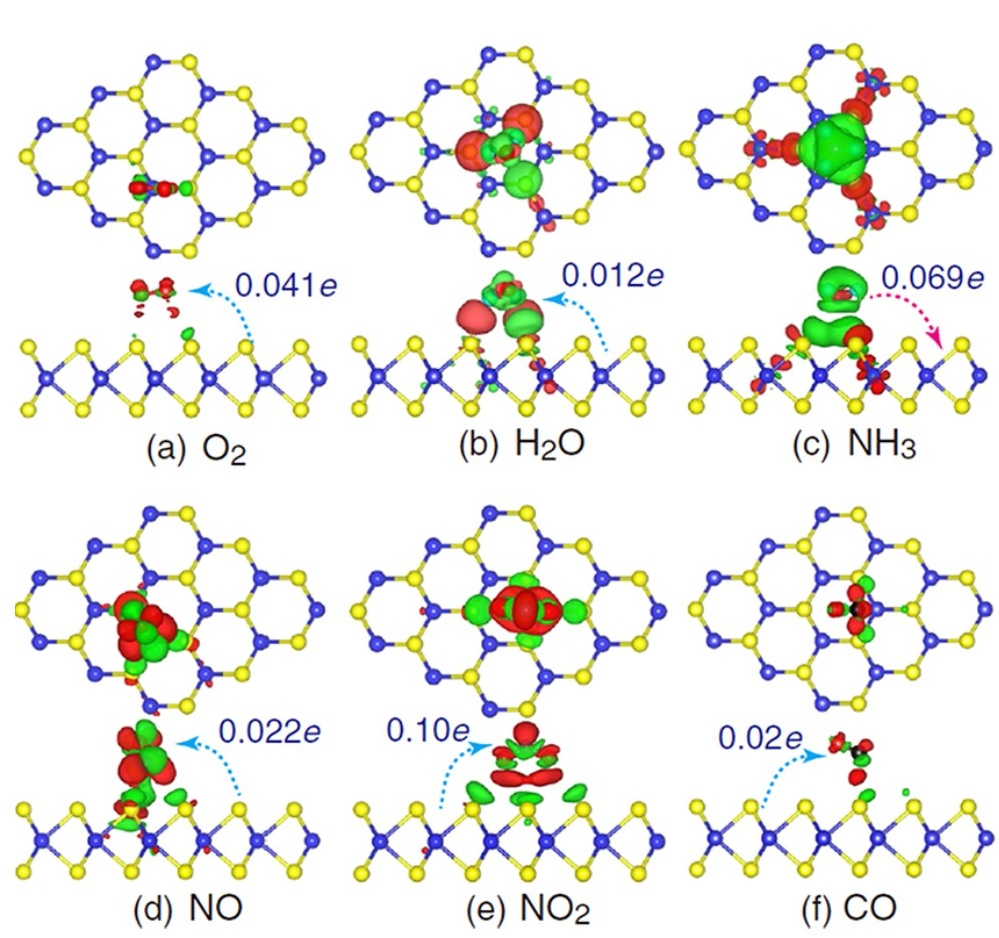
\includegraphics[width=\textwidth]{02_functionality/fig/charge_density_change.jpg}
    \caption{}
    \label{fig:charge_density}
\end{subfigure}
\caption{(\subref{fig:adsorption_process}) Depiction of the adsorption of different gases onto a MoS2 surface. \cite{Lee2018} (\subref{fig:charge_density}) Change of the charge density during the adsoprtion of different gases. Green(red) refers to positve(negative) changes of the charge density. \cite{Lee2018}}
\label{fig:adsorption}
\end{figure}

There are multiple techniques that amplify the performance metrics of 2D gas sensors. The most straight forward approach is to heat the active regions of the gas sensor, in order to achieve better response times. However, this method is undesirable in most applications, as it produces additional challenges in fabrication and increases the passive energy consumption of the sensor drastically. A more sophisticated approach is, for instance, the targeted pollution of the sensor structure. This introduces accumulation points for the analyte, which increases the adsorption rate of the gas and thus the sensitivity of the sensor. \\
Another possibility is to stack the 2D structure vertically with another material. This would create a heterojunction. Since \glspl{tmd} are semiconductors, it is possible to stack them in a p-n manner, effectively creating a space charge region that further depopulates the device of charge carries. The charge carrier density modulations induced by adsorbed gas therefore creates a greater effect on the conductivity of the sensor. \\ 
In \cite{Gu2018} it is shown that the sensitivity of 2D \gls{tmd} based gas sensors can doubled, when \Gls{uv} light is shone onto the sensor surface. This effect can be tied to the photo generation and recombination of electron/hole pairs and charge transfer.
